%!TEX root = ../dissertation.tex
\chapter{OpenCog System} \label{cha:opencog_system}

The OpenCog design aims to capture the spirit of the architecture and dynamics of the brain without imitating the details (which are largely unknown) via:
\begin{itemize}
	\item Integrating together a carefully selected combination of cognitive algorithms acting on different kinds of knowledge.
	\item A scalable, robust and flexible C++ software architecture.
	\item A manner specifically designed:
	\begin{itemize}	
	\item To cooperate together with “cognitive synergy” for the scope of tasks characteristic of human intelligence. 
	\item To give rise to the emergence of an effectively functioning knowledge network in the AI system’s mind, as it interacts with the world, including a self-updating hierarchical/heterarchical ontology and models of itself and others.
	\end{itemize}
\end{itemize}
Following section, Section \ref{sec:cognitive_synergy}, elaborates on the new concepts introduced in these points.


\section{Cognitive Synergy}\label{sec:cognitive_synergy}

OpenCog is a diverse assemblage of cognitive algorithms, each embodying its own innovations. The power of the overall architecture is its careful adherence to the principle of Cognitive Synergy. \\
The human brain consists of a host of subsystems that perform particular tasks, both specialized and general in nature, connected together in a manner enabling them to synergetically assist, rather than work against each other. \\
The essential principles of Cognitive Synergy Theory (CST) can be summarized in the following points, further explored in \cite{inproceedings_cognitive_synergy}:

\begin{enumerate}
	\item Intelligence can be understood as the ability to achieve complex goals in a certain set of environments. 
	\item An intelligent system requires a "multi-memory" architecture, meaning the possession of a number of specialized yet interconnected knowledge types.
	\item "Cognitive processes": a system must possess knowledge creation mechanisms corresponding to each of these memory types.
	\item Each cognitive process must have the ability to recognize when it lacks information and thus, draw it from knowledge creation mechanisms related to other types of knowledge.
	\item The Cognitive Synergy is, therefore, represented by the interaction between the knowledge creation mechanisms, which perform much more effectively in combination than non-interactive mode. 
	\item The activity of the different cognitive processes involved in an intelligent system can be modeled in terms of the schematic implication "Context \& Procedure $\rightarrow$ Goal".
\end{enumerate}

These points are implicit in the systems theory of mind given in \cite{goertzel2006the}, where more thorough characterizations of these ideas can be found.\\
Interactions as mentioned in Points 4 and 5 are the conceptual core of CST. \\
Most AI algorithms suffer from combinatorial explosions. In a “general intelligence” context, there is a lack of intrinsic constraint; consequently, the algorithms are unable to filter through all the possibilities (as opposed to a ANI problem like chessplaying, where the context is huge but constrained and hence restricts the scope of possible combinations that needs to be considered). \\
To decrease the severity of combinatorial explosions, one can use an AGI architecture based on CST, in which the different learning mechanisms dealing with a certain sort of knowledge, are designed to synergize with ones dealing with other sorts of knowledge. \\
It is necessary that each learning mechanism recognizes when it is "blocked" and then, it can ask for help to the other complementary cognitive mechanisms. \\
The Figure \ref{fig:cognitive_processes} is proposed to give a general visual idea of these concepts. It shows an overview of the most important cognitive dynamics considered in Cognitive Synergy Theory and describes the behavior of a system as it pursues a set of goals, which are then refined by inference (through a logic engine or as an emergent process resulting from the dynamics of an Neural Network system), aided by other processes. \\
%Attualmente il progetto OpenCog è in via di sviluppo e parte dei concetti presentati qui potrebbero essere obsoleti, migliorati o evoluti.

\begin{figure}
\centering
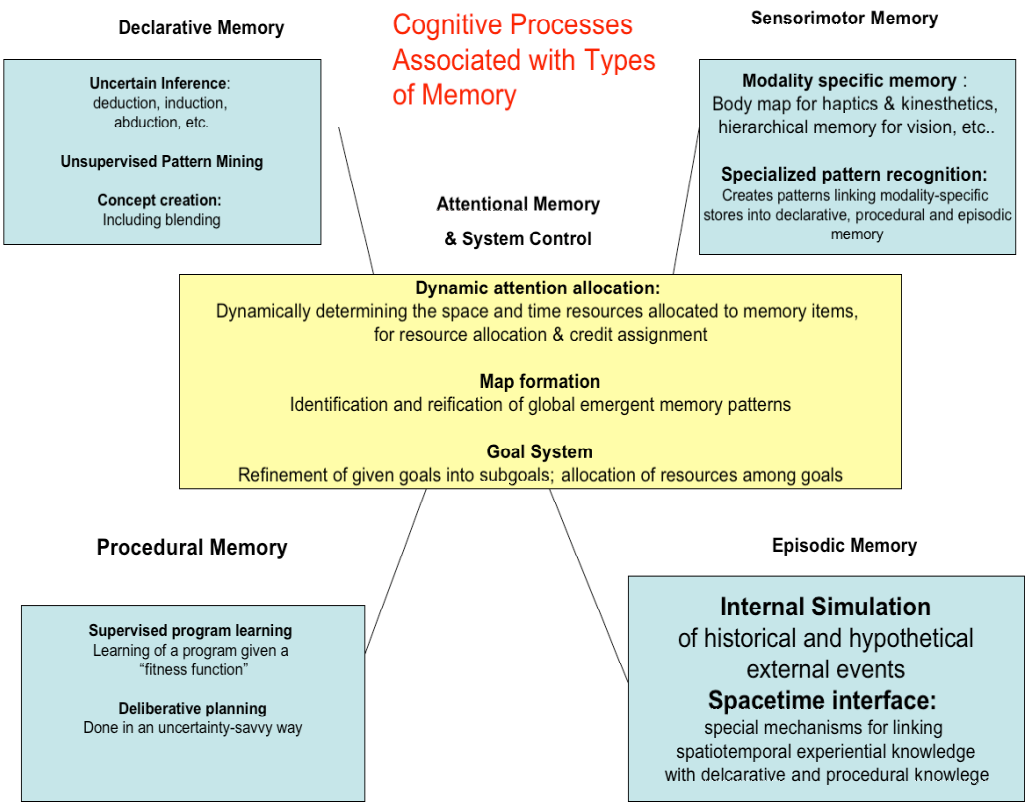
\includegraphics[width=0.7
\textwidth]{figures/Magistrale/04 - cognitive_processes_and_memory}
\caption[Cognitive Processes.]{A high-level overview of the main types of cognitive process considered in Cognitive Synergy Theory, categorized according to the type of knowledge with which each process deals.
\label{fig:cognitive_processes}}
\end{figure} 

The detailed argument as to why we think our selection of cognitive algorithms and our integration methods will have the desired effect, is sketched on the OpenCog wiki site (\footnotesize{\url{https://wiki.opencog.org/w/Background_Publications}}\normalsize) and various previously-published conference papers, and has been presented more thoroughly (from a more particular perspective) in the 2014 books Engineering General Intelligence vol. 1 and 2 \cite{DBLP:series/atlantis/GoertzelPG14, DBLP:series/atlantis/GoertzelPG14a}.


\section{History}\label{sec:history}

Patternist systems theory of intelligence SMEPH-based intelligence \cite{inproceedings_SMEPH}

In order to put this architecture to work, we have crafted a roadmap based on roughly mimicking the environment and development of young human children. A series of child-level learning tasks has been carefully laid out, which may be manifested via either virtual world agents or physical robots, and which lead from infant-level capabilities up to the grade school level. These tasks cover all the major cognitive capabilities displayed by young humans, and involve the integration of all major aspects of human intelligence, including perception, action, cognition, learning, memory, creativity, socialization, language, self-modeling, etc.

% OpenCog Development Roadmap https://wiki.opencog.org/w/OpenCog_Development_Roadmap
\cite{DBLP:series/atlantis/Rohde10}

\section{Atomspace}\label{sec:atomspace}


\section{Atomese}\label{sec:atomese}


\section{Reasons}\label{sec:reasons}